\documentclass{article}
\title{Jeu CHSH}
\usepackage{amsmath}
\usepackage{graphicx}
\usepackage{amsfonts}
\graphicspath{ {./} }


\author{CAO Trong Nhan, Julien Hofmann}
\date{ 8 Mars 2023}


\begin{document}
\maketitle

\section{Presenter le jeu CHSH}

\subsection{Une partie de histoire:}

Bien que Eistein soit un des contributeur plus significatifs de la quantum mécanisme, certaines phénomènes quantiques ne sont pas approuvés par lui, notamment intrication quantique. Donc, Einstein a développé le paradoxe EPR en 1935 avec Podolsky et Rosen avec le premise que il existe des variables cachées locales, qui sont possible de calculer si nous connaissons le propriété et l'environnement locale de système. Il s'applle réalisme locale.
\\Cependant, en 1964, John S.Bell a réclamé que réalisme locale n'est pas compatible avec le mecanisme quantique, au moins avec le système quantique à cette époque. Bell a indiqué des modèles qui donne des limites dans le système locale de Einstein (Bell inégalité) mais être violés dans le système quantique. Après quelque années, Clauser, Horne, Shimony et Holt ont donné la version plus compact et simple de Bell inégalité, qui s'appelle CHSH inégalité.

\subsection{La principe du jeu CHSH:}

Dans ce jeu, il y a 2 participants Alice (A) et Bob (B), qui sont séparés (par une espace suffisament loins ou l'isolement, etc) pour éviter la communication direct mutuellement. Il existe aussi un arbitre qui peut donner des \textit{questions} et verifier des \textit{responses} de deux participants. D'abord, l'abitre presente à chaque paricipant un valeur binaire séparement (1 ou 0). On note ces valeurs x pour Alice et y pour Bob. A et B doivent après aussi choisir un valeur binaire (a et b). Bien sur, Alice ne sais pas b et Bob ne sais pas a. Ils gagnent si $a \oplus b = xy$. Par exemple, si $x = y = 0$ et $a = b = 1$, A et B gagnent le jeu.
\\\textbf{\underline{Remarque:}} $a \oplus b = x$ telle que $x \in \{0,1\}$ et $x \equiv a + b \pmod{n}$. Eventuellement, pour des fonctions logiques comme dans le jeu, c'est le fonction XOR. Quand même, $xy$ est la fonction ET. Donc, le nature de jeu CHSH et de changer la fonction ET à XOR.
\begin{figure}[h]
\centering
\includegraphics[scale = 0.5]{Simplify model}
\centering
\caption{Modèle simplifié du jeu}
\end{figure}
\\Le problèmes est Alice et Bob peuvent choisir leurs réponses après l'abitre a donné des questions. Plus, A et B peuvent aussi discuter avant pour avoir le mieux strategie. L'arbitre est aussi équitable et il donne des questions aléatoires complètement. Donc, quel est le mieux strategie?


\section{Les stratégies pour le réalisme locale}

\subsection{Stratégie déterministe (sans probabilité):}

Pour A, il peut choisir entre 4 stratégies: 

\[
\left\{
\begin{aligned}
a &= 1 \\
a &= 0 \\
a &= x \\
a &= \bar{x}
\end{aligned}
\right.
\]

Nous notons cette stratégie $g(x)$. Le cas pour B est idem et nous le notons $h(y)$. Dans ce cas de  stratégie déterministe, A et B choisissent absolutement une stratégie pour le reste du jeu (c'est-à-dire ils ne peuvent pas changer des stratégies). Nous avons 4 pairs différentes de x et y, donc, il y a 4 possibilités pour chaque pair de stratégies. Cependant, il exist toujour 1 sur 4 possibilités que Alice et Bob perdent le jeu dans tous cas. Par contradiction, nous supposons que:

\begin{center}
$\exists g: \{0;1\} \rightarrow \{0;1\}$ et $\exists h: \{0;1\} \rightarrow \{0;1\}$:
\\$\forall \{x;y\} \in \{0;1\}^2: g(x) \oplus h(y) = xy$ 
\\$\Rightarrow 1 = 1.1 = h(1) \oplus g(1) = (h(1) \oplus g(0)) \oplus (g(0) \oplus h(0)) \oplus (h(0) \oplus g(1)) = (1.0) \oplus (0.0) \oplus (0.1) = 0 \oplus 0 \oplus 0 = 0 \Rightarrow$ Absurd
\end{center}

En effet, nous pouvons indiquer le cas échoué pour tous 16 pairs de stratégies. 
\begin{figure}[h]
\centering
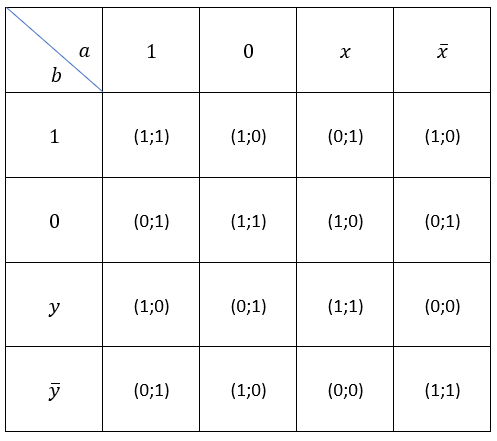
\includegraphics[scale = 0.5]{Table}
\centering
\caption{Des pairs échoués (x;y)}
\end{figure}
\\Nous considerons que l'arbitre est complètement équitable, donc, la possibilité de chaque cas est la même (25\%). Autrement dit, la chance de gagner le jeu de Bob et Alice ne peut pas dépasser 75\%. En effet, si Alice et Bob choisissent des stratégies a = b = 0, dans 3 cas sur 4, xy = 0 alors ils gagnent. 


\subsection{Stratégie classique(avec probabilité):}

Maintenant, nous voulons généraliser le stratégie par la probabilité. Il y a des possibilités pour choisir des sratégies différents. Nous fixons $(x,y) \in \{0;1\}^2$. Pour Alice, nous notons $X_a (x,y)$ son stratégie et $\alpha(X_a (x,y))$ la possibilité de choisir cette stratégie. Idem pour $X_b(x,y)$ et $\beta(X_b (x,y))$. Soit $\mathcal{G} (x,y)$ la possibilité de gagner avec $(x,y) \in \{0;1\}^2$
\end{document}